%% SW design: klassebeskrivelse SPI API

\begin{figure}[htbp] \centering
{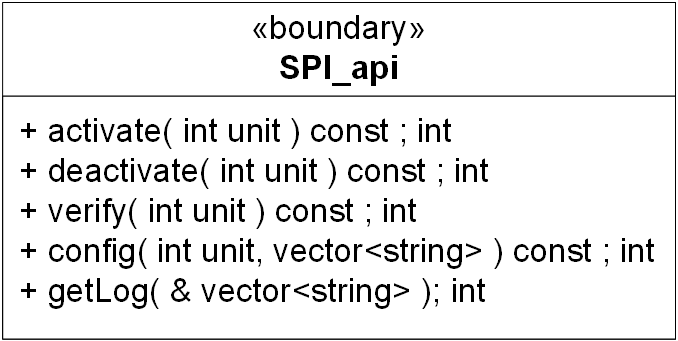
\includegraphics[scale=1.5]{filer/design/Klassediagrammer/SPI_API}}
\caption{klassediagram SPI API}
\label{fig:SPI API klassediagram}
\end{figure} 

{\centering
\textbf{SPI\_api klasse}\par
}
\textbf{Ansvar:} At være det lag imellem applications laget og device driver laget. Skal håndtere snakken med device driveren til SPI kommunikation \\

int activate( int unit ) const \\
\textbf{Parametre:} modtager en integer på følgende enhed som skal aktiveres \\
\textbf{Returværdi:} returnere en integer som er 0 hvis operationen gik godt. Ved fejl returneres en negativ integer i overenstemmelse med fejl-listen \\
\textbf{Beskrivelse:} metoden skal kunne aktivere enheden som er identificeret ved integeren den modtager. Hvis dette går godt returneres 0, ellers returneres en fejlkode i overenstemmelse med fejl-listen.\\

int deactivate( int unit ) const \\
\textbf{Parametre:}  modtager en integer på følgende enhed som skal deaktiveres\\
\textbf{Returværdi}: returnere en integer som er 0 hvis operationen gik godt. Ved fejl returneres en negativ integer i overenstemmelse med fejl-listen  \\
\textbf{Beskrivelse:} metoden skal kunne deaktivere enheden som er identificeret ved integeren den modtager. Hvis dette går godt returneres 0, ellers returneres en fejlkode i overenstemmelse med fejl-listen.\\

int verify( int unit ) const \\
\textbf{Parametre:}  modtager en integer på følgende enhed som skal verificerese\\
\textbf{Returværdi:} returnere en integer som er 0 hvis operationen gik godt. Ved fejl returneres en negativ integer i overenstemmelse med fejl-listen  \\
\textbf{Beskrivelse:} metoden skal kunne verificere om en enhed, identificeret ved integeren den modtager, er på SPI nettet. Hvis dette går godt returneres 0, ellers returneres en fejlkode i overenstemmelse med fejl-listen.\\

int config( int unit, vector<string> ) const \\
\textbf{Parametre:} modtager en integer på følgende enhed som skal konfigureres. Derudover modtager den en vector af typen string som indeholder parametrene enheden skal konfigureres med \\
\textbf{Returværdi:} returnere en integer som er 0 hvis operationen gik godt. Ved fejl returneres en negativ integer i overenstemmelse med fejl-listen  \\
\textbf{Beskrivelse:} metoden skal kunne sende konfigurations parametre ud til enheder ved hjælp af device driverne til SPI kommunikationen. Hvis dette går godt returneres 0, ellers returneres en fejlkode i overenstemmelse med fejl-listen.\\

int getLog( \& vector<string>  ) \\
\textbf{Parametre:}  modtager en referance til en vector af typen string som loggen skal lægges over i.\\
\textbf{Returværdi:} returnere en integer som er 0 hvis operationen gik godt. Ved fejl returneres en negativ integer i overenstemmelse med fejl-listen  \\
\textbf{Beskrivelse:} metoden skal kunne hente log fra alle enheder på SPI netværket og gemme dem i den modtaget vector. \\








